\documentclass[12pt,a4paper]{article}
\usepackage[utf8]{inputenc}
\usepackage{amsmath}
\usepackage{amsfonts}
\usepackage{amssymb}
\usepackage{graphicx}
\usepackage[hidelinks]{hyperref}
\usepackage{booktabs}
\usepackage{longtable}
\usepackage{geometry}
\usepackage{fancyhdr}
\usepackage{caption}
\usepackage{subcaption}
\usepackage{listings}
\usepackage{xcolor}
\usepackage{float}
\usepackage{array}
\usepackage{multirow}
\usepackage{tikz}
\usetikzlibrary{shapes.geometric, arrows, positioning, fit}

\geometry{margin=1in}
\setlength{\headheight}{14.5pt}
\pagestyle{fancy}
\fancyhf{}
\rhead{Bike Rental Analysis}
\lhead{Business Intelligence}
\rfoot{\thepage}

% Define colors for code listings
\definecolor{codegreen}{rgb}{0,0.6,0}
\definecolor{codegray}{rgb}{0.5,0.5,0.5}
\definecolor{codepurple}{rgb}{0.58,0,0.82}
\definecolor{backcolour}{rgb}{0.95,0.95,0.92}

% Hyperref setup
\hypersetup{
    colorlinks=true,
    linkcolor=blue,
    filecolor=magenta,
    urlcolor=cyan,
    pdftitle={Bike Rental Demand Forecasting Dashboard},
    pdfpagemode=FullScreen,
}

% Code listing style
\lstdefinestyle{mystyle}{
    backgroundcolor=\color{backcolour},
    commentstyle=\color{codegreen},
    keywordstyle=\color{magenta},
    numberstyle=\tiny\color{codegray},
    stringstyle=\color{codepurple},
    basicstyle=\ttfamily\footnotesize,
    breakatwhitespace=false,
    breaklines=true,
    captionpos=b,
    keepspaces=true,
    numbers=left,
    numbersep=5pt,
    showspaces=false,
    showstringspaces=false,
    showtabs=false,
    tabsize=2
}

\lstset{style=mystyle}

\begin{document}

\begin{titlepage}
\centering
\textbf{Universit\`a degli Studi di Napoli Federico II}\\
\textbf{Data Science}\\[10mm]

Business Intelligence \break

\begin{figure}[h!]
\begin{center} 
\includegraphics[height=8cm]{figures/uni-logo.png}
\end{center}
\end{figure}

\textbf{Zain Abbas} \\[2mm]
\textbf{Airaf Siddiqui} \\[2mm]
\textbf{Adil Shahzad} \\[2cm]

\textbf{Bike Rental Demand Forecasting: A Time Series Analysis Dashboard with Machine Learning} \\[5mm]

Project Report\\[1cm]

\textbf{FLORA AMATO}\\
\null\vfill

Naples, \the\year

\end{titlepage}

\newpage

\tableofcontents

\newpage

\listoffigures
\listoftables

\newpage

\begin{abstract}
This report presents the design, implementation, and evaluation of an interactive Streamlit dashboard for bike rental demand forecasting. The system analyzes two years of hourly bike rental data (17,451 records) from a bike-sharing system, implementing comprehensive time series analysis, exploratory data analysis, and machine learning-based forecasting. Key contributions include: (1) a four-page interactive dashboard with real-time data exploration capabilities; (2) discovery of data leakage in the original model that artificially inflated performance metrics (R$^2$ = 0.9999); and (3) development of a realistic Random Forest model achieving R$^2$ = 0.9456 using only weather and calendar features. The analysis reveals significant patterns: 82.5\% of users are registered subscribers, casual users show 93.4\% demand reduction during storms compared to 56.3\% for registered users, and hourly demand varies by a factor of 77 between peak (5 PM) and off-peak (4 AM) hours. The dashboard provides time series decomposition, autocorrelation analysis, PCA, and multi-model comparison capabilities for decision support.

\textbf{Keywords:} Time Series Analysis, Demand Forecasting, Machine Learning, Random Forest, Streamlit Dashboard, Bike-Sharing Systems, Data Leakage Detection
\end{abstract}

\newpage

\section{Introduction}

\subsection{Background and Motivation}

Bike-sharing systems have emerged as an important component of urban transportation infrastructure, offering an environmentally sustainable alternative to motor vehicles while addressing first-mile and last-mile connectivity challenges. These systems generate substantial data on usage patterns, creating opportunities for data-driven optimization of fleet distribution, maintenance scheduling, and capacity planning.

Accurate demand forecasting is critical for bike-sharing operations for three primary reasons:

\begin{enumerate}
    \item \textbf{Fleet Rebalancing}: Predicting demand enables proactive redistribution of bikes to stations where they will be needed, reducing instances where users cannot find available bikes.
    \item \textbf{Maintenance Planning}: Understanding temporal patterns helps schedule maintenance during low-demand periods, minimizing service disruption.
    \item \textbf{Capacity Investment}: Long-term demand trends inform decisions about expanding or contracting fleet size and station infrastructure.
\end{enumerate}

This project addresses the challenge of building an interactive analytical tool that enables stakeholders to explore historical patterns and generate demand forecasts using machine learning models.

\subsection{Project Scope and Objectives}

This project develops a comprehensive Streamlit dashboard for bike rental analysis with the following scope:

\begin{itemize}
    \item \textbf{Data Analysis}: Interactive exploration of two years of hourly bike rental data
    \item \textbf{Time Series Analysis}: Decomposition, autocorrelation analysis, and stationarity testing
    \item \textbf{Machine Learning}: Random Forest-based demand forecasting with model comparison
    \item \textbf{Decision Support}: KPI tracking and weather impact analysis for operational decisions
\end{itemize}

The primary objectives are:
\begin{enumerate}
    \item Develop a multi-page Streamlit dashboard with interactive visualizations
    \item Implement time series analysis methods (decomposition, ACF/PACF, PCA)
    \item Train and evaluate machine learning models for demand forecasting
    \item Identify and address data leakage issues in model development
    \item Provide actionable insights for bike-sharing system operators
\end{enumerate}

\subsection{Contributions}

This work makes the following contributions:
\begin{enumerate}
    \item \textbf{Interactive Dashboard}: A four-page Streamlit application with real-time data exploration, forecasting simulation, and model comparison capabilities
    \item \textbf{Data Leakage Discovery}: Identification of critical data leakage issues (lag features and user-type decomposition) that inflated model performance from R$^2$ = 0.9999 to a realistic R$^2$ = 0.9456
    \item \textbf{Comprehensive Analysis}: Integration of EDA, time series decomposition, autocorrelation analysis, and PCA in a unified platform
    \item \textbf{User Segmentation Insights}: Quantification of behavioral differences between registered (82.5\%) and casual (17.5\%) users, particularly regarding weather sensitivity
    \item \textbf{Reproducible Methodology}: Documented approach for building time series forecasting dashboards with proper feature engineering
\end{enumerate}

\section{Literature Review and Background}

\subsection{Bike-Sharing Demand Forecasting}

Bike-sharing demand forecasting has received significant attention in transportation research. Borgnat et al. \cite{borgnat2011shared} demonstrated that bike-sharing usage exhibits strong temporal patterns correlated with commuting hours, weather conditions, and day of week. More recent work by Xu et al. \cite{xu2018bike} applied gradient boosting methods to achieve improved prediction accuracy by incorporating external factors.

Key factors influencing bike rental demand include:
\begin{itemize}
    \item \textbf{Temporal Features}: Hour of day, day of week, month, season, holidays
    \item \textbf{Weather Conditions}: Temperature, humidity, wind speed, precipitation
    \item \textbf{User Type}: Registered subscribers vs. casual users exhibit different behaviors
\end{itemize}

\subsection{Time Series Analysis Methods}

Classical time series analysis provides foundational techniques for understanding temporal data:

\begin{itemize}
    \item \textbf{Seasonal Decomposition}: Separates time series into trend, seasonal, and residual components \cite{cleveland1990stl}
    \item \textbf{Autocorrelation Analysis}: ACF and PACF plots identify lag dependencies and guide model selection for ARIMA-type models
    \item \textbf{Stationarity Testing}: Augmented Dickey-Fuller (ADF) test determines whether differencing is required
\end{itemize}

\subsection{Machine Learning for Forecasting}

Random Forest regression has proven effective for demand forecasting due to its ability to capture non-linear relationships and handle mixed feature types without extensive preprocessing \cite{breiman2001random}. Key advantages include:
\begin{itemize}
    \item Implicit feature selection through importance scores
    \item Robustness to outliers and missing values
    \item No assumption of linear relationships
    \item Built-in cross-validation through out-of-bag error
\end{itemize}

\subsection{Interactive Dashboard Development}

Streamlit has emerged as a leading framework for building data science applications, offering rapid prototyping with Python-native syntax \cite{streamlit2024}. Key features relevant to this project include:
\begin{itemize}
    \item Session state management for cross-page data sharing
    \item File upload widgets for dynamic data and model loading
    \item Integration with Plotly for interactive visualizations
    \item Caching mechanisms for performance optimization
\end{itemize}

\section{System Architecture}

\subsection{Overall System Design}

The dashboard follows a multi-page architecture with centralized data management through Streamlit's session state:

\begin{figure}[H]
\centering
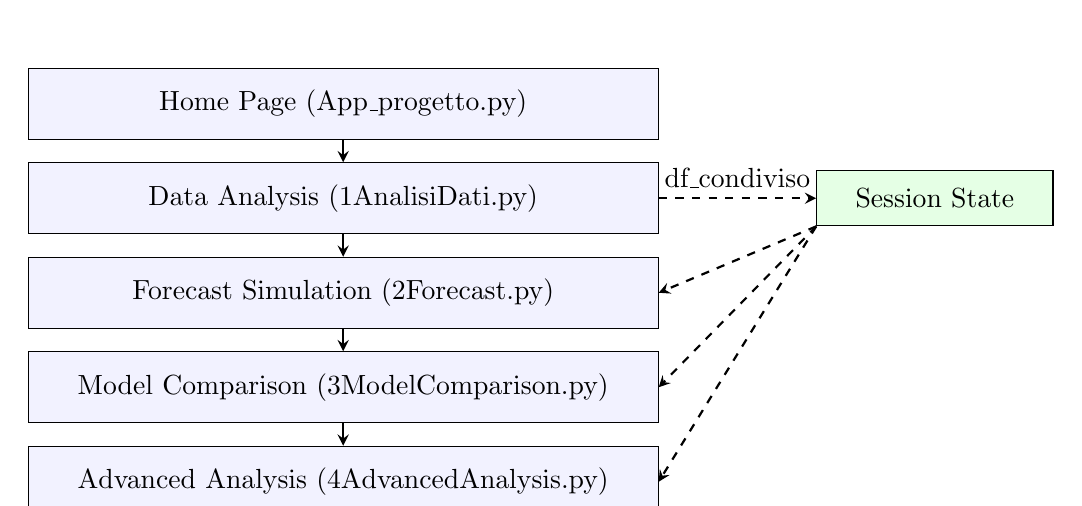
\begin{tikzpicture}[
    node distance=1.2cm,
    box/.style={rectangle, draw, minimum width=8cm, minimum height=0.9cm, align=center, fill=blue!5},
    arrow/.style={->, >=stealth, thick}
]
    % Nodes
    \node[box] (home) {Home Page (App\_progetto.py)};
    \node[box, below of=home] (data) {Data Analysis (1AnalisiDati.py)};
    \node[box, below of=data] (forecast) {Forecast Simulation (2Forecast.py)};
    \node[box, below of=forecast] (compare) {Model Comparison (3ModelComparison.py)};
    \node[box, below of=compare] (advanced) {Advanced Analysis (4AdvancedAnalysis.py)};

    % Session State
    \node[rectangle, draw, minimum width=3cm, minimum height=0.7cm, fill=green!10, right=2cm of data] (state) {Session State};

    % Arrows
    \draw[arrow] (home) -- (data);
    \draw[arrow] (data) -- (forecast);
    \draw[arrow] (forecast) -- (compare);
    \draw[arrow] (compare) -- (advanced);
    \draw[arrow, dashed] (data.east) -- (state.west) node[midway, above] {df\_condiviso};
    \draw[arrow, dashed] (state.south west) -- (forecast.east);
    \draw[arrow, dashed] (state.south west) -- (compare.east);
    \draw[arrow, dashed] (state.south west) -- (advanced.east);
\end{tikzpicture}
\caption{Dashboard Architecture with Session State Data Flow}
\label{fig:architecture}
\end{figure}

\subsection{Page Modules}

The system implements four specialized page modules:

\begin{table}[H]
\centering
\caption{Dashboard Page Modules}
\begin{tabular}{llp{6cm}}
\toprule
\textbf{Page} & \textbf{Purpose} & \textbf{Key Features} \\
\midrule
Data Analysis & EDA and KPIs & CSV upload, efficiency metrics, user composition, weather impact, peak hours heatmap \\
Forecast & Prediction Simulation & Model loading, time slider, real-time prediction display \\
Model Comparison & Multi-Model Evaluation & Multiple model upload, RMSE/MAE/R$^2$/MAPE metrics, prediction overlay \\
Advanced Analysis & Statistical Methods & Decomposition, ACF/PACF, PCA, stationarity test \\
\bottomrule
\end{tabular}
\label{tab:pages}
\end{table}

\subsection{Data Flow and Session State}

Data sharing between pages uses Streamlit's session state mechanism:

\begin{lstlisting}[language=Python, caption=Session State Data Sharing]
# Page 1: Store uploaded data
st.session_state['df_condiviso'] = df

# Other pages: Retrieve shared data
if 'df_condiviso' not in st.session_state:
    st.warning("Load data first in Data Analysis page")
    st.stop()
df = st.session_state['df_condiviso']
\end{lstlisting}

\subsection{Technology Stack}

\begin{table}[H]
\centering
\caption{Technology Stack}
\begin{tabular}{ll}
\toprule
\textbf{Component} & \textbf{Technology} \\
\midrule
Dashboard Framework & Streamlit \\
Data Processing & Pandas, NumPy \\
Visualization & Plotly, Matplotlib \\
Machine Learning & scikit-learn (Random Forest) \\
Time Series Analysis & statsmodels \\
Model Persistence & joblib \\
\bottomrule
\end{tabular}
\label{tab:tech}
\end{table}

\section{Data Exploration}

\subsection{Dataset Description}

The analysis uses the Capital Bikeshare dataset containing hourly bike rental records:

\begin{table}[H]
\centering
\caption{Dataset Overview}
\begin{tabular}{lc}
\toprule
\textbf{Metric} & \textbf{Value} \\
\midrule
Total Records & 17,451 \\
Date Range & 2011-01-02 to 2012-12-31 \\
Total Days & 730 \\
Temporal Resolution & Hourly \\
\bottomrule
\end{tabular}
\label{tab:dataset}
\end{table}

Key features include temporal variables (hour, day, month, season, holiday, working day), weather conditions (temperature, humidity, wind speed, weather situation), and target variables (total rentals, registered users, casual users).

\subsection{User Composition Analysis}

Analysis of user types reveals a significant imbalance between registered and casual users:

\begin{table}[H]
\centering
\caption{User Composition Metrics}
\begin{tabular}{lcc}
\toprule
\textbf{User Type} & \textbf{Total Rentals} & \textbf{Percentage} \\
\midrule
Registered & 2,672,729 & 82.5\% \\
Casual & 619,773 & 17.5\% \\
\midrule
\textbf{Total} & \textbf{3,292,502} & \textbf{100\%} \\
\bottomrule
\end{tabular}
\label{tab:users}
\end{table}

\begin{figure}[H]
\centering
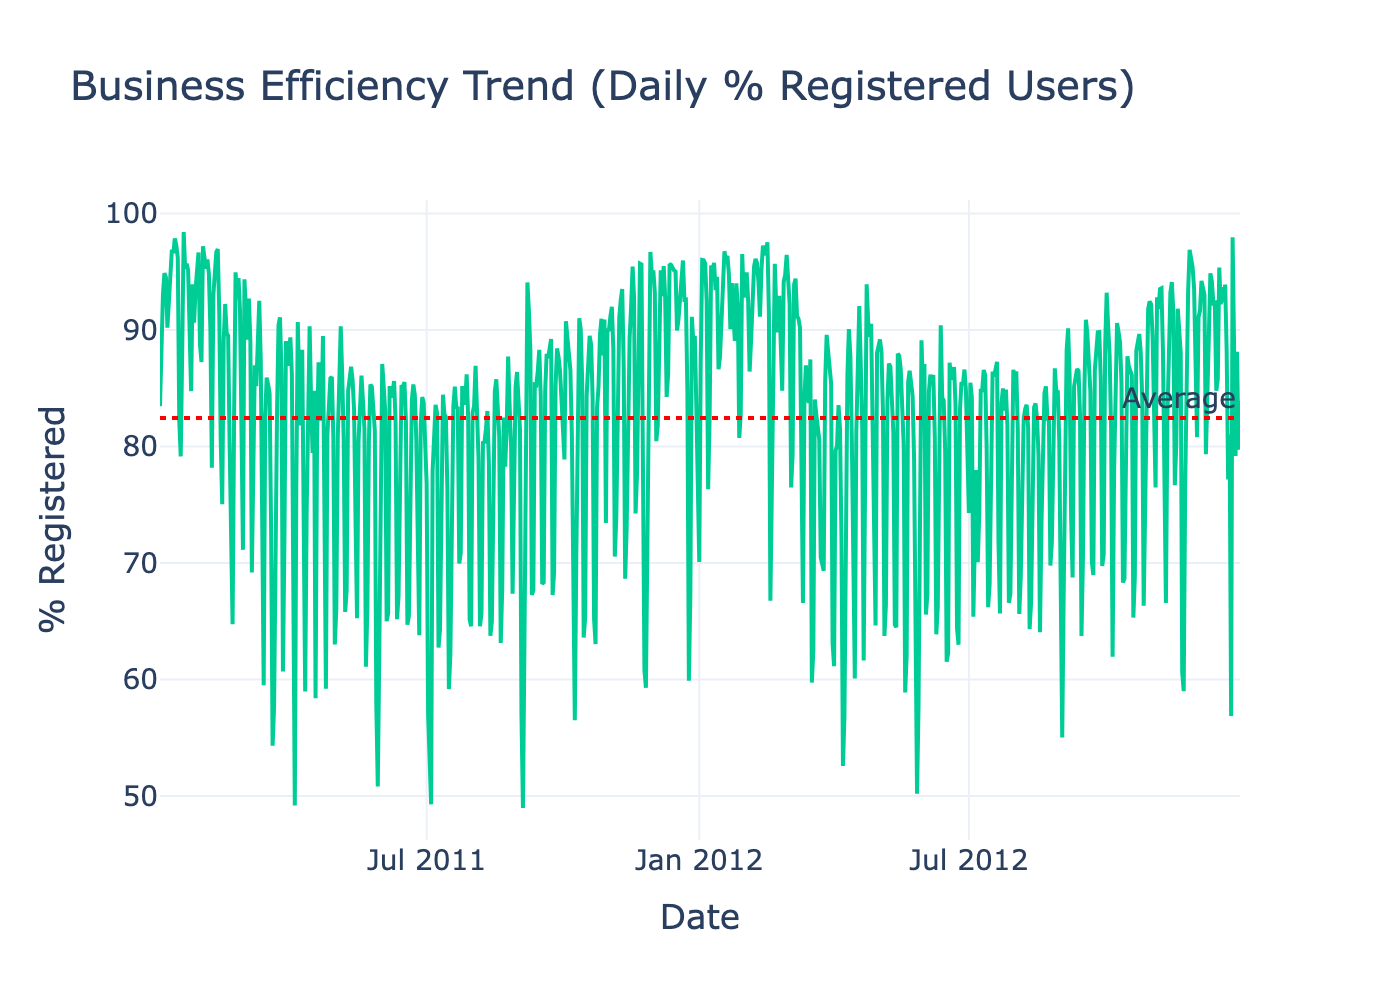
\includegraphics[width=0.85\textwidth]{figures/01_efficiency_trend.png}
\caption{Daily Efficiency Rate (Registered Users Percentage). The trend shows consistent dominance of registered users at approximately 82.5\%, indicating a stable subscriber base with predictable commuting patterns.}
\label{fig:efficiency}
\end{figure}

\begin{figure}[H]
\centering
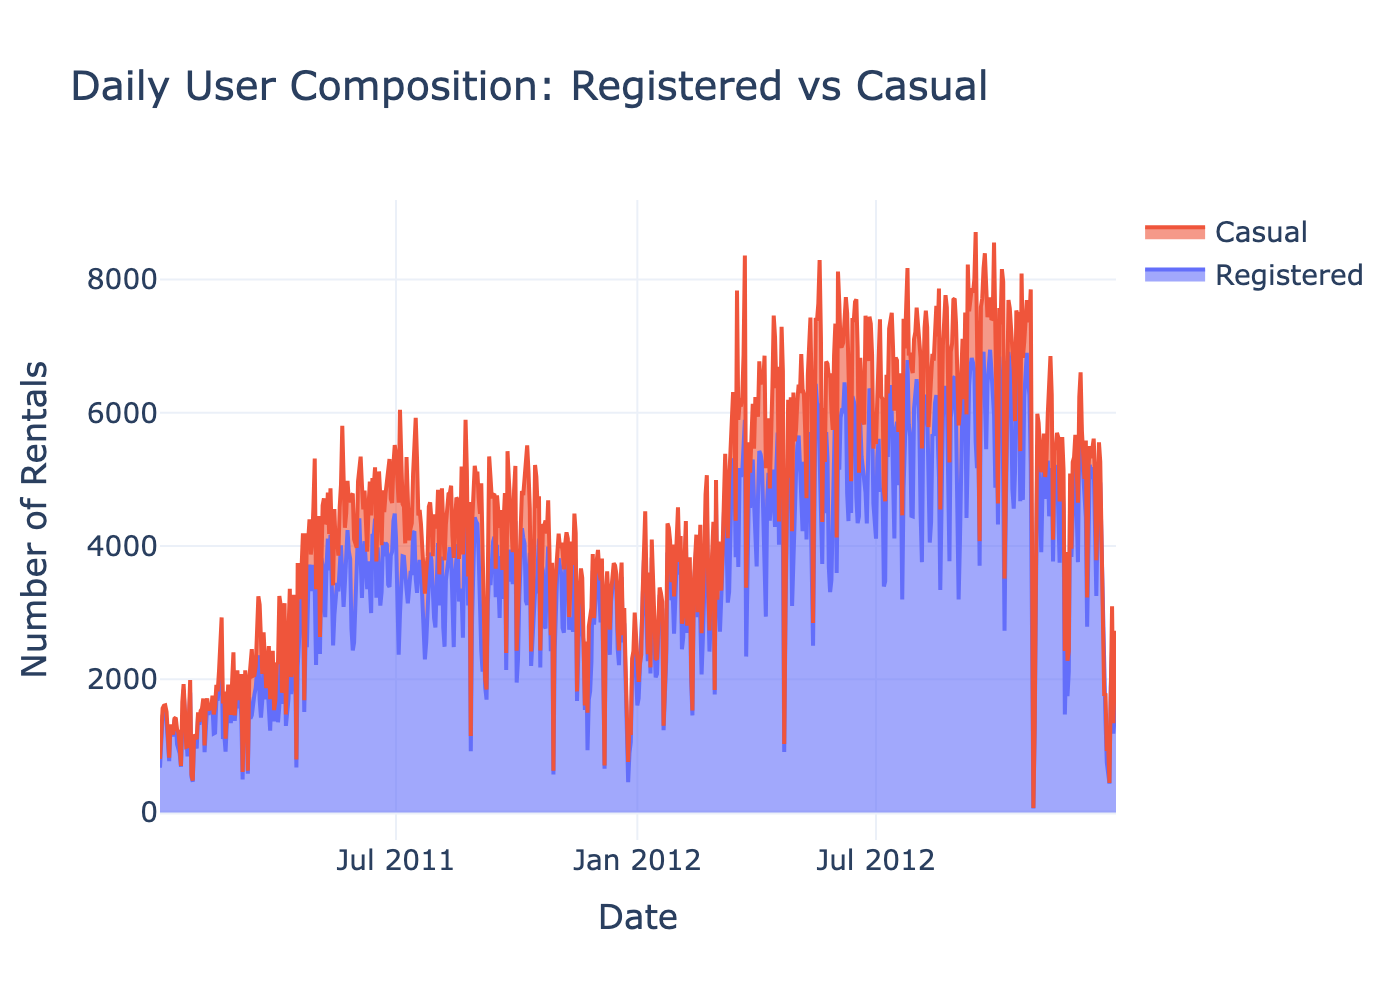
\includegraphics[width=0.85\textwidth]{figures/02_subscribers_vs_casual_area.png}
\caption{User Composition Over Time. Stacked area chart showing the daily volume of registered (blue) and casual (orange) users, demonstrating seasonal patterns with higher usage in summer months.}
\label{fig:composition}
\end{figure}

\begin{figure}[H]
\centering
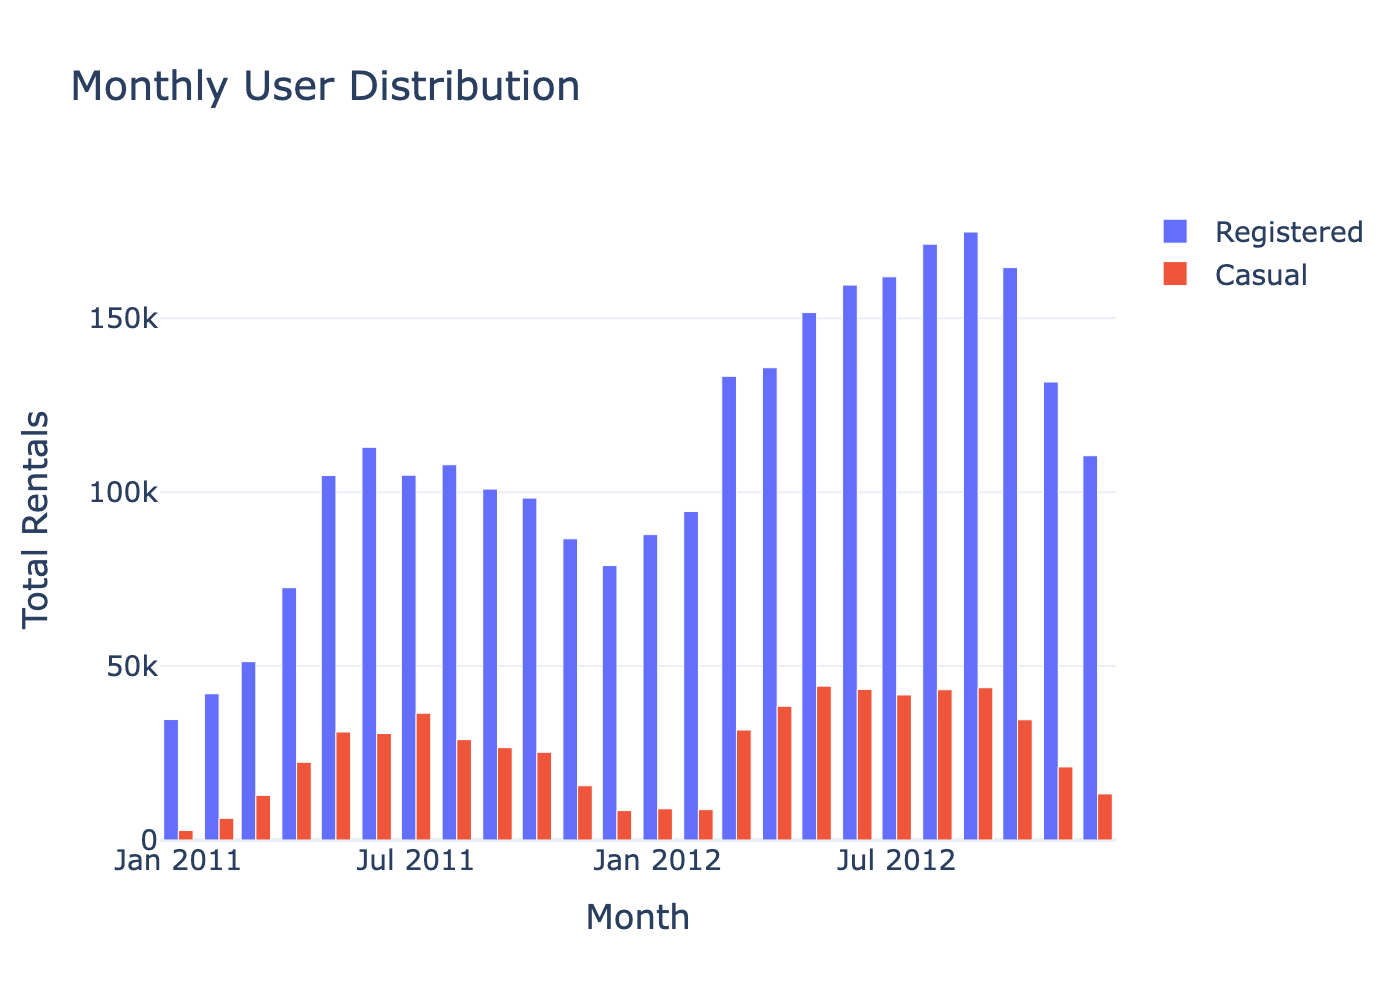
\includegraphics[width=0.85\textwidth]{figures/03_monthly_user_distribution.png}
\caption{Monthly Distribution by User Type. Bar chart showing monthly rental volumes with clear seasonal peaks in summer (June-September) and lower demand in winter months.}
\label{fig:monthly}
\end{figure}

\subsection{Weather Impact Analysis}

Weather conditions significantly influence bike rental demand, with differential effects on user types:

\begin{table}[H]
\centering
\caption{Weather Sensitivity by User Type}
\begin{tabular}{lcc}
\toprule
\textbf{User Type} & \textbf{Demand Drop (Sunny to Storm)} & \textbf{Interpretation} \\
\midrule
Registered & 56.3\% & Less sensitive (essential trips) \\
Casual & 93.4\% & Highly sensitive (recreational) \\
\bottomrule
\end{tabular}
\label{tab:weather}
\end{table}

\begin{figure}[H]
\centering
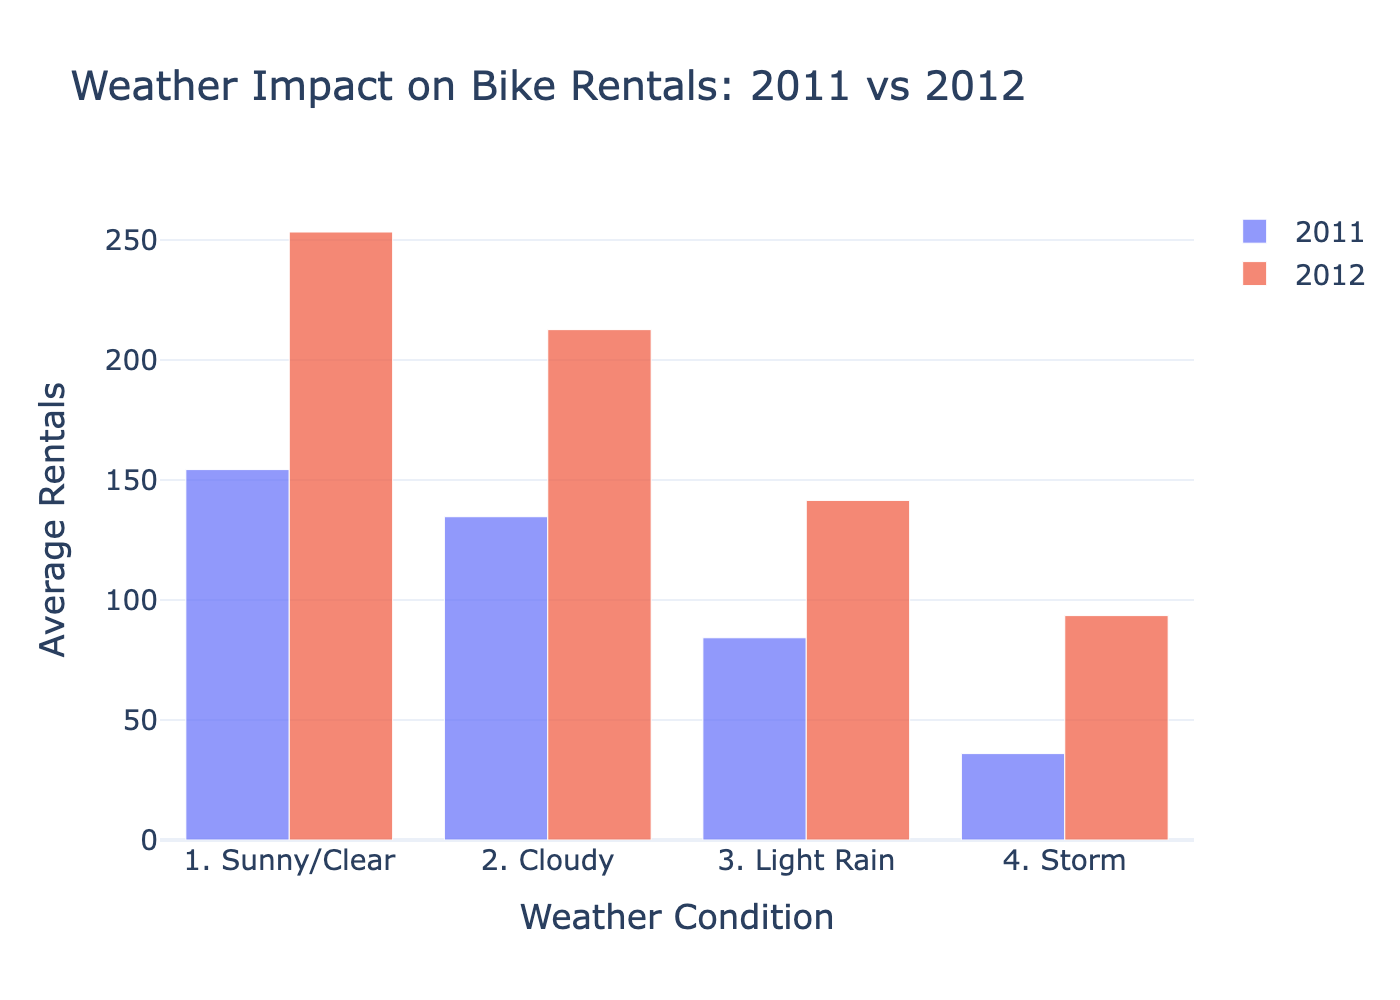
\includegraphics[width=0.85\textwidth]{figures/04_weather_impact_yearly.png}
\caption{Weather Impact Comparison (2011 vs 2012). Grouped bar chart showing average rentals by weather condition across both years, demonstrating consistent weather sensitivity patterns.}
\label{fig:weather_year}
\end{figure}

\begin{figure}[H]
\centering
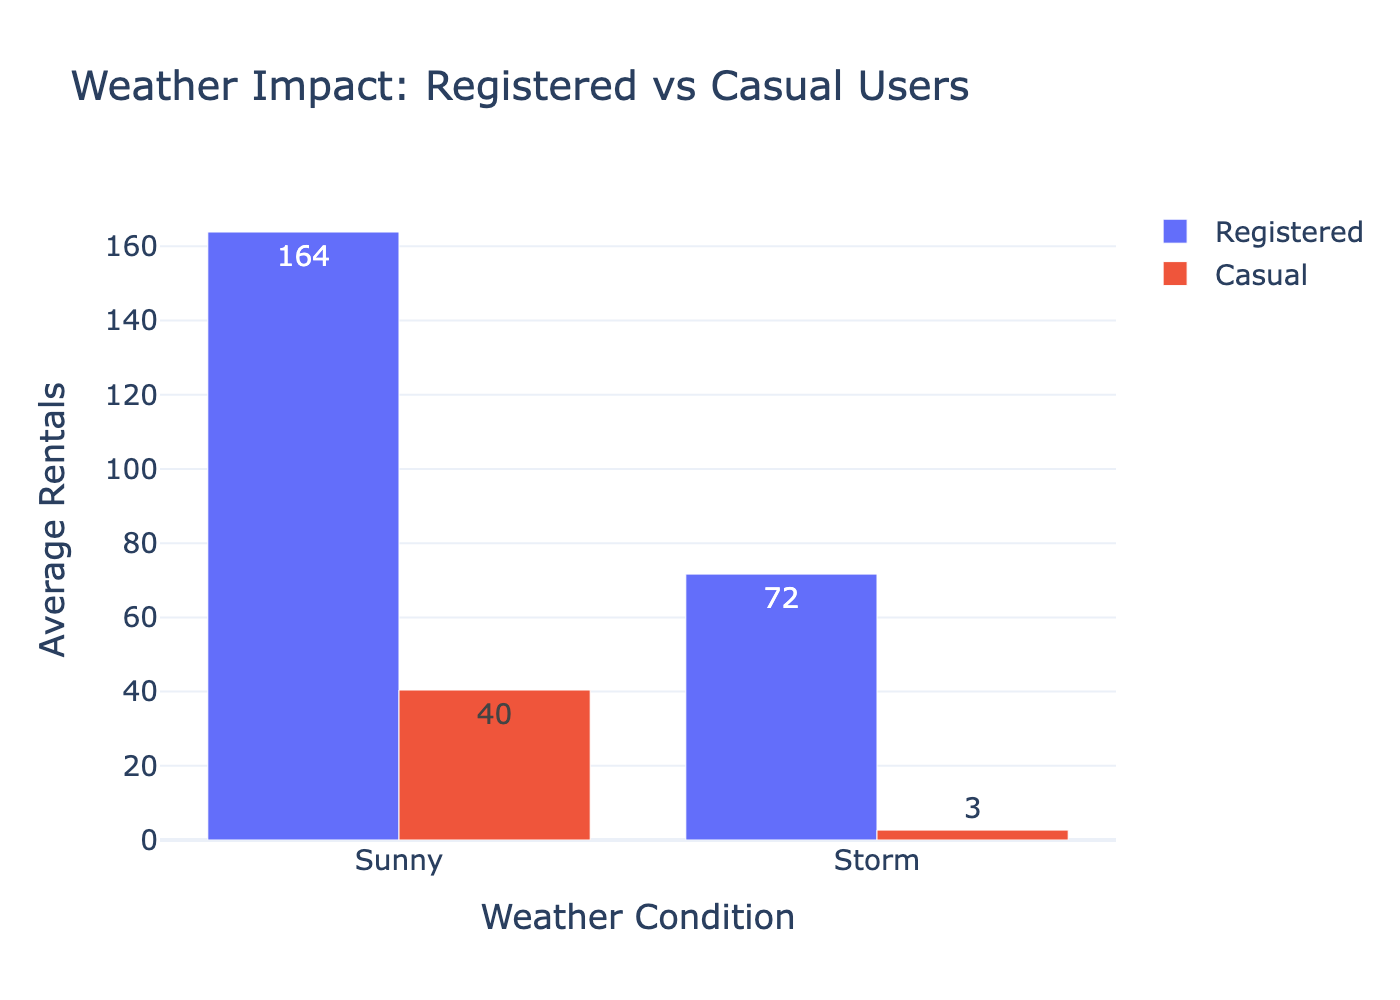
\includegraphics[width=0.85\textwidth]{figures/05_climate_impact_user_type.png}
\caption{Climate Sensitivity by User Type. Comparison showing casual users experience 93.4\% demand reduction during storms compared to 56.3\% for registered users, indicating registered users make essential trips regardless of weather.}
\label{fig:weather_user}
\end{figure}

\subsection{Temporal Patterns}

Analysis of hourly patterns reveals distinct usage profiles:

\begin{table}[H]
\centering
\caption{Peak Hour Analysis}
\begin{tabular}{lcc}
\toprule
\textbf{Period} & \textbf{Hour} & \textbf{Average Rentals} \\
\midrule
Peak & 17:00 (5 PM) & 462 \\
Off-Peak & 04:00 (4 AM) & 6 \\
\midrule
\textbf{Ratio} & & \textbf{77x} \\
\bottomrule
\end{tabular}
\label{tab:peak}
\end{table}

\begin{figure}[H]
\centering
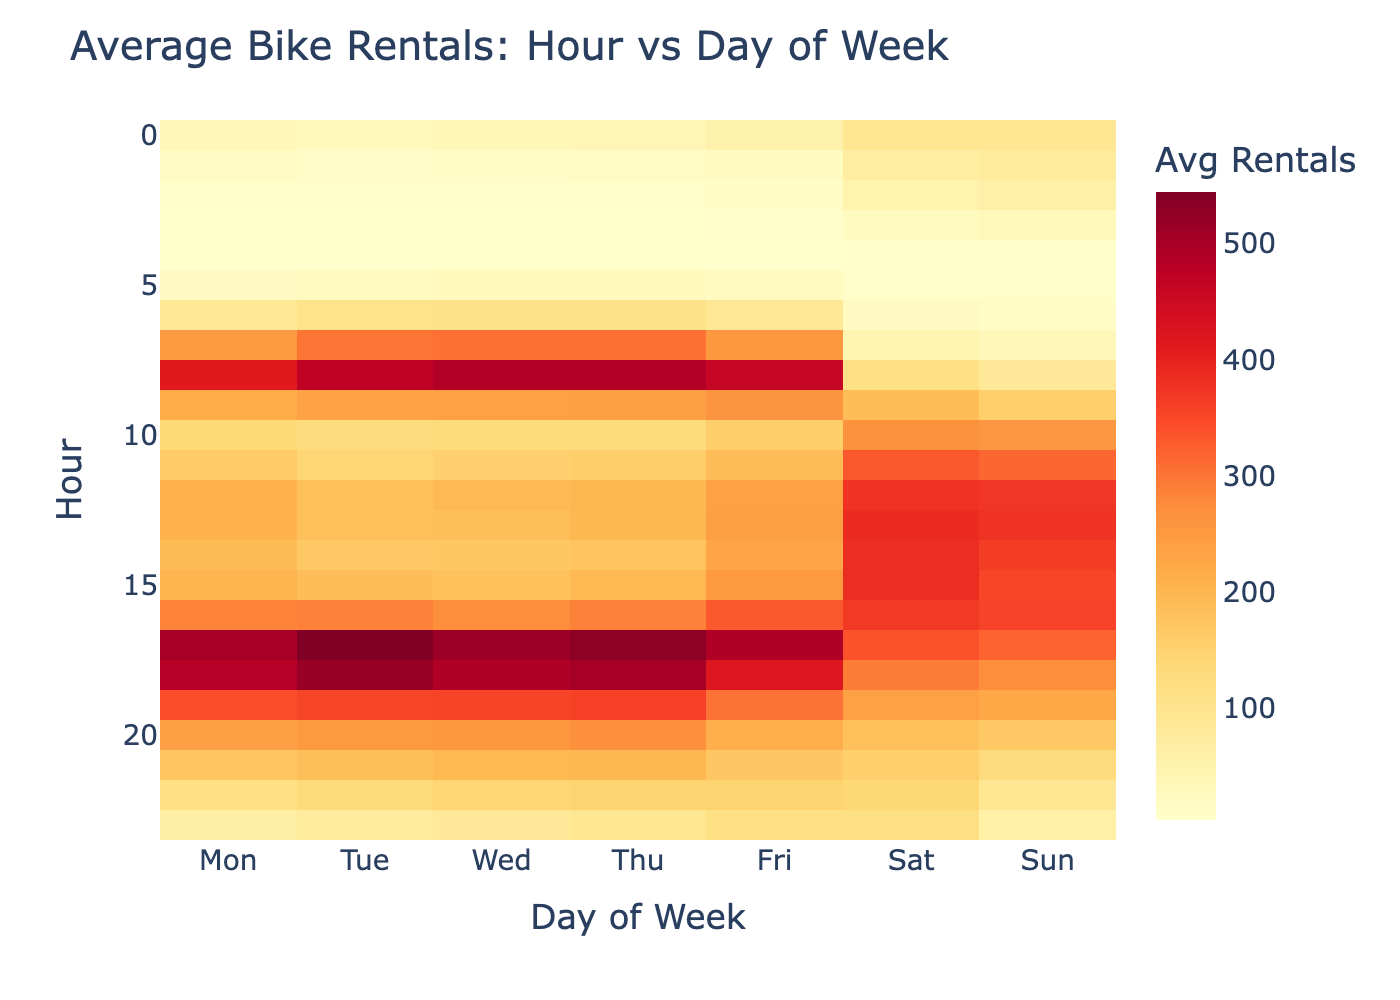
\includegraphics[width=0.85\textwidth]{figures/06_peak_hours_heatmap.png}
\caption{Hourly Demand Heatmap. Hour-by-day-of-week visualization showing clear commuting patterns on weekdays (peaks at 8 AM and 5-6 PM) versus gradual midday increases on weekends.}
\label{fig:heatmap}
\end{figure}

\section{Time Series Analysis}

\subsection{Working Day vs Non-Working Day Patterns}

Distinct usage patterns emerge between working and non-working days:

\begin{figure}[H]
\centering
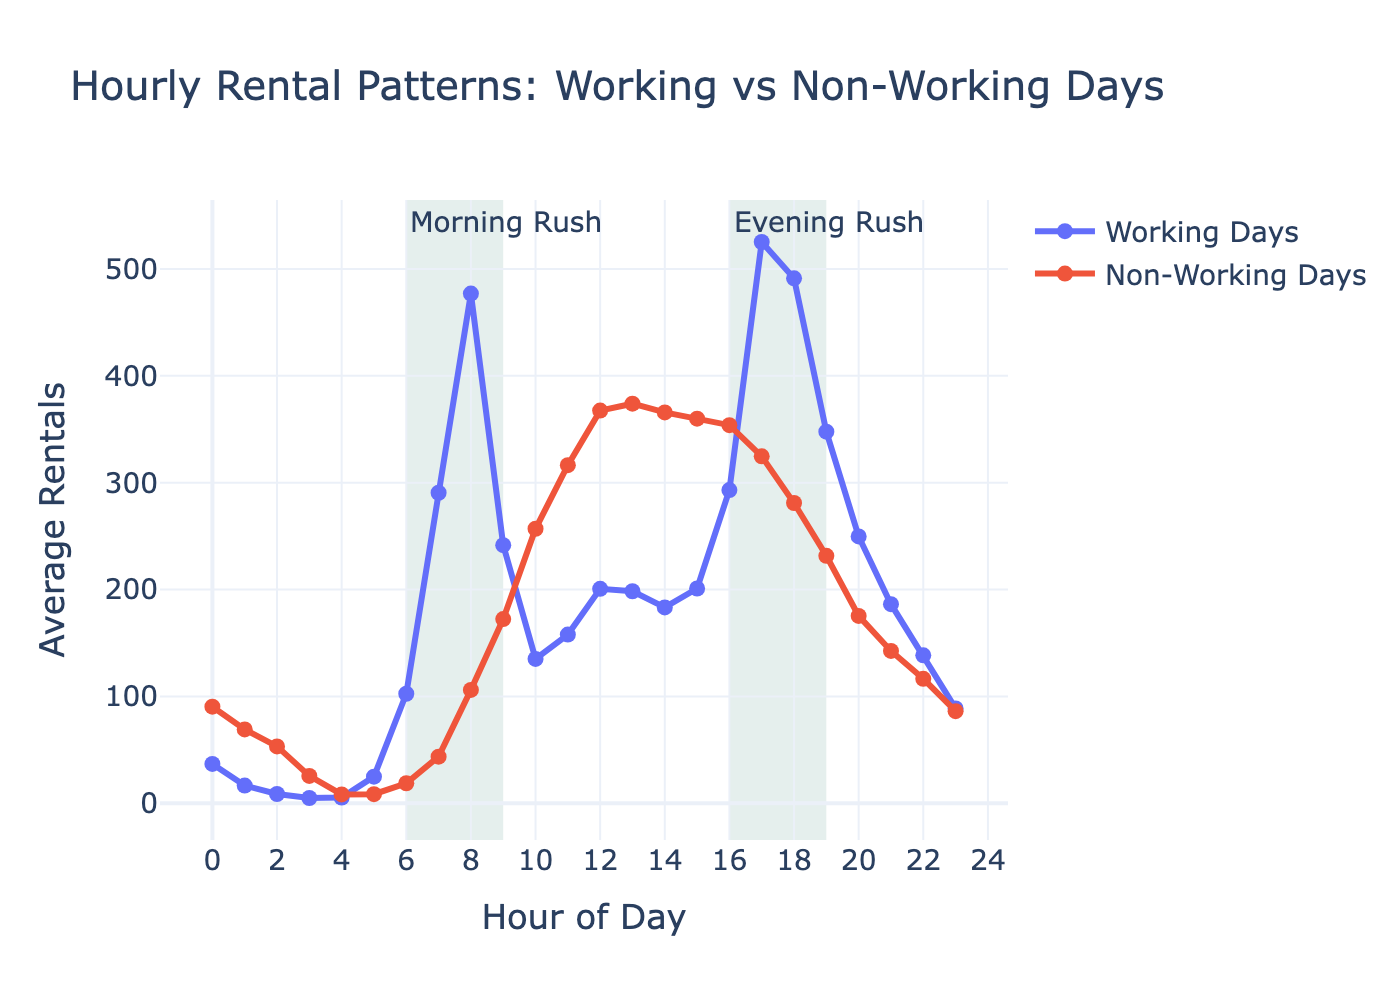
\includegraphics[width=0.85\textwidth]{figures/07_working_vs_nonworking.png}
\caption{Working Day vs Non-Working Day Patterns. Working days show bimodal distribution with peaks at 8 AM and 5-6 PM (commuting), while non-working days exhibit unimodal distribution peaking around midday (recreational use).}
\label{fig:working}
\end{figure}

\subsection{Time Series Decomposition}

Seasonal decomposition separates the time series into interpretable components:

\begin{figure}[H]
\centering
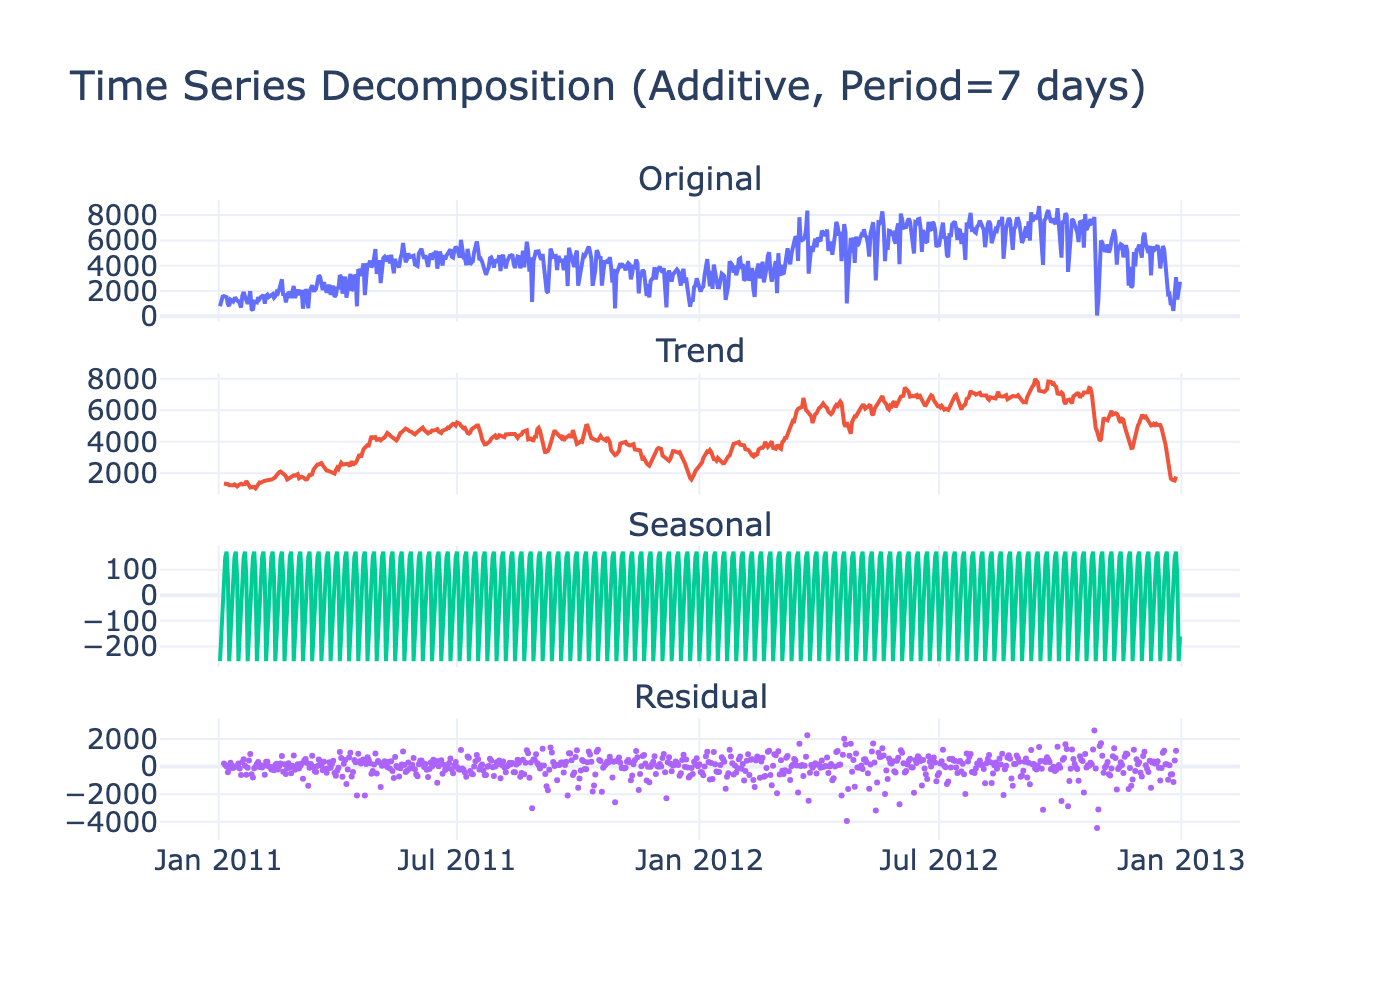
\includegraphics[width=0.85\textwidth]{figures/10_decomposition.png}
\caption{Time Series Decomposition. Four-panel visualization showing: (1) Original series with clear seasonality; (2) Upward trend indicating growing bike-share adoption; (3) Seasonal component capturing weekly patterns; (4) Residuals representing unexplained variation.}
\label{fig:decomp}
\end{figure}

\subsection{Autocorrelation Analysis}

ACF and PACF analysis reveals significant lag dependencies:

\begin{figure}[H]
\centering
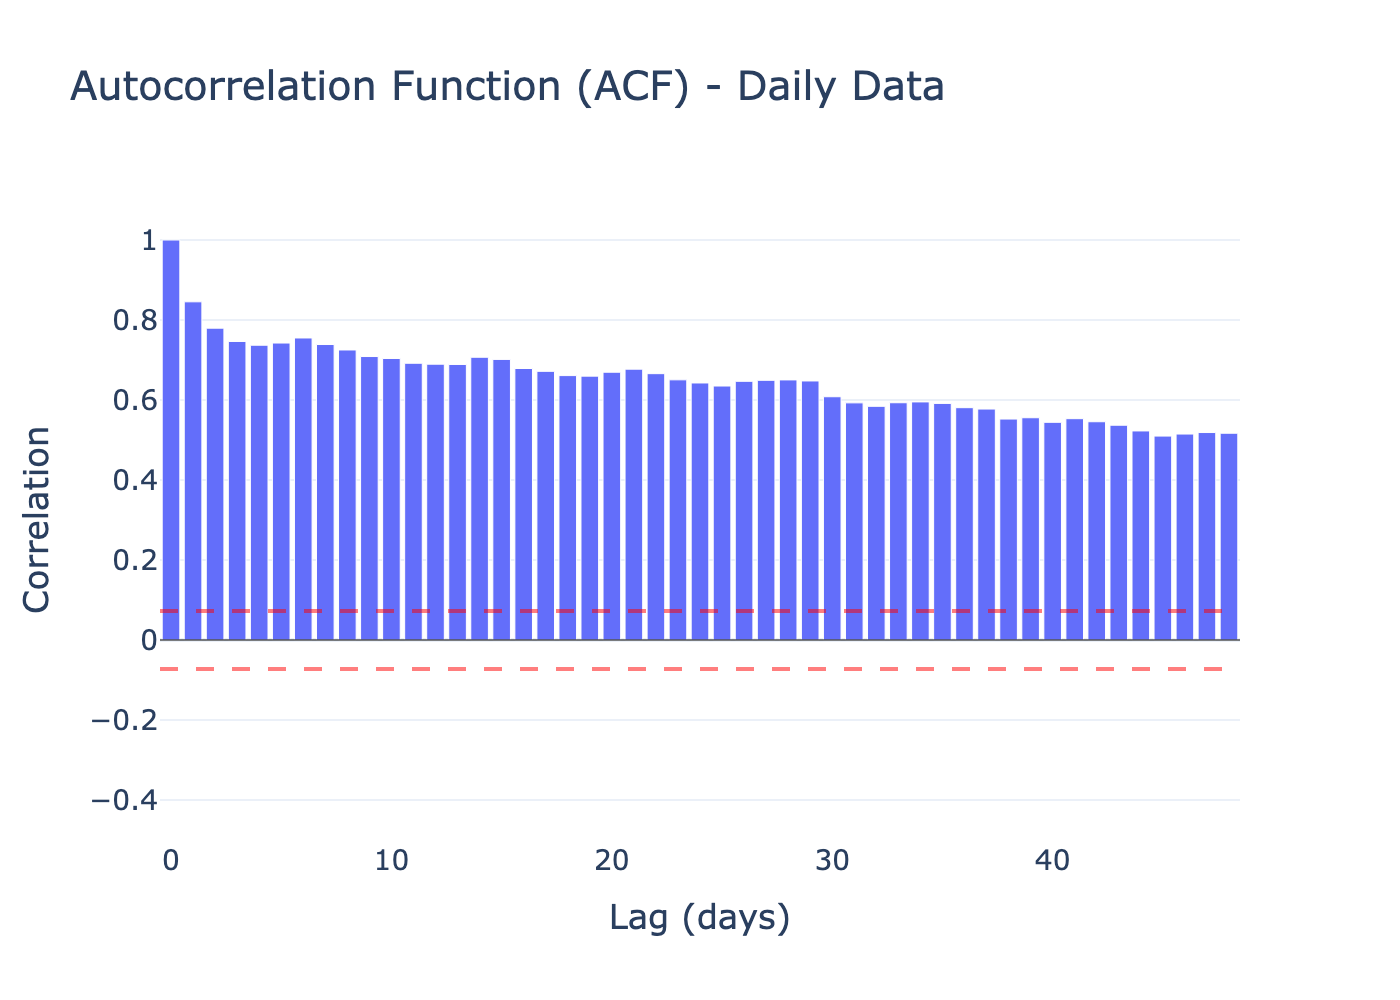
\includegraphics[width=0.85\textwidth]{figures/11_acf_plot.png}
\caption{Autocorrelation Function (ACF). Significant correlations at lag 1 (immediate dependency), lag 24 (daily cycle), and lag 168 (weekly cycle) confirm strong temporal patterns suitable for forecasting.}
\label{fig:acf}
\end{figure}

\begin{figure}[H]
\centering
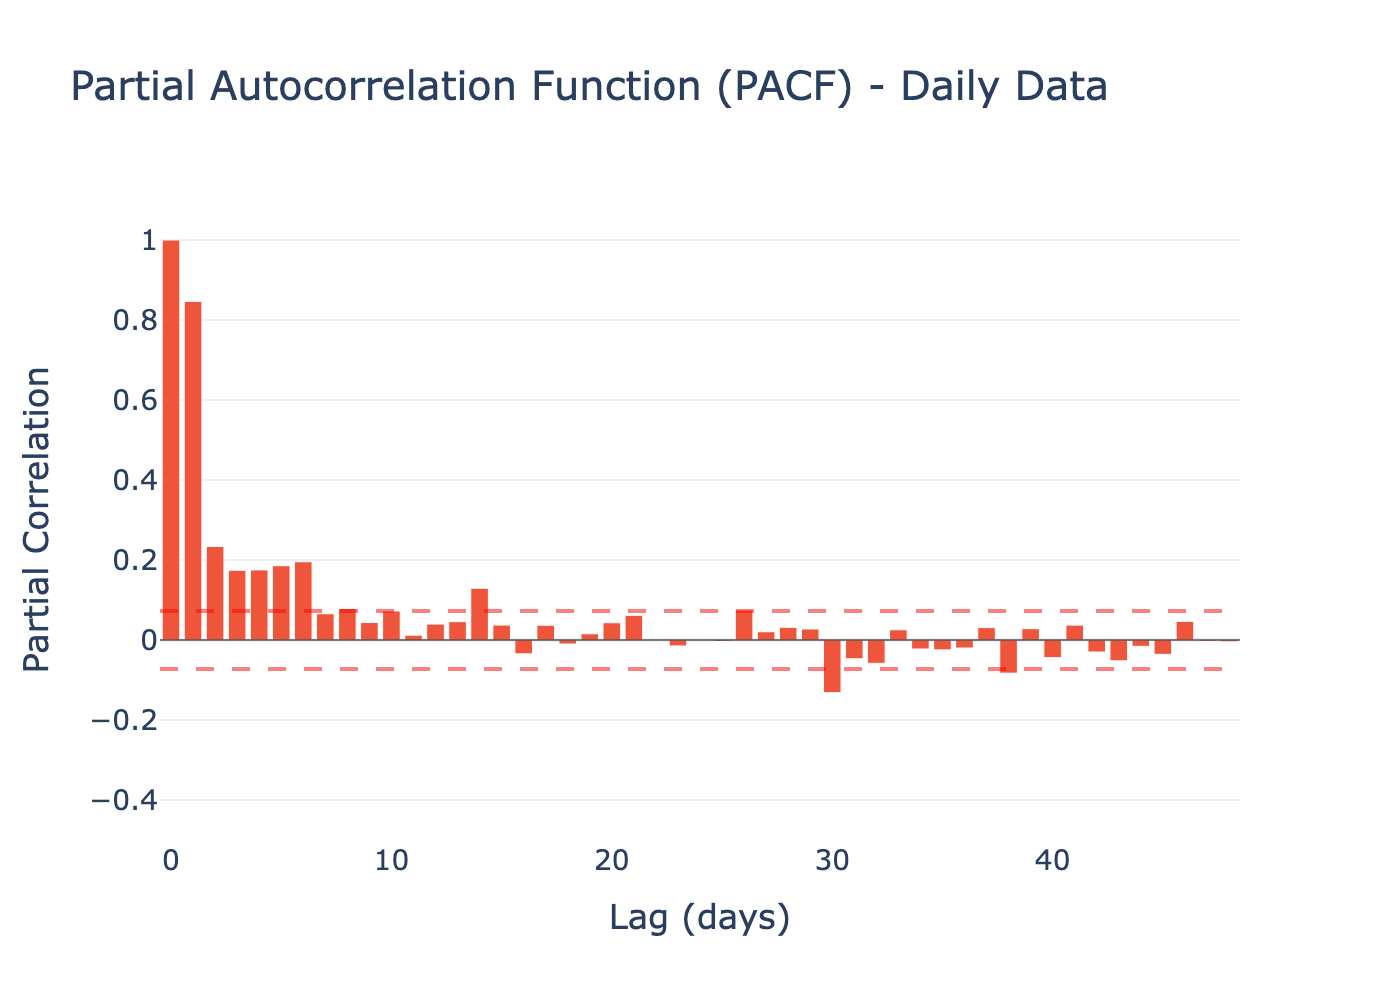
\includegraphics[width=0.85\textwidth]{figures/12_pacf_plot.png}
\caption{Partial Autocorrelation Function (PACF). Sharp cutoff after lag 2 with significant spikes at seasonal lags suggests AR components would be appropriate for ARIMA modeling.}
\label{fig:pacf}
\end{figure}

Key findings from autocorrelation analysis:
\begin{itemize}
    \item \textbf{Lag 1}: Strong immediate correlation (yesterday affects today)
    \item \textbf{Lag 24}: Daily cycle correlation in hourly data
    \item \textbf{Lag 168}: Weekly pattern (7 days $\times$ 24 hours)
\end{itemize}

\section{Feature Engineering}

\subsection{Principal Component Analysis}

PCA was applied to weather-related features to understand dimensionality:

\begin{table}[H]
\centering
\caption{PCA Explained Variance}
\begin{tabular}{lccc}
\toprule
\textbf{Component} & \textbf{Variance} & \textbf{Cumulative} & \textbf{Interpretation} \\
\midrule
PC1 & 49.9\% & 49.9\% & Temperature variation \\
PC2 & 32.2\% & 82.1\% & Humidity/wind patterns \\
PC3 & 17.6\% & 99.7\% & Residual weather variation \\
\bottomrule
\end{tabular}
\label{tab:pca}
\end{table}

\begin{figure}[H]
\centering
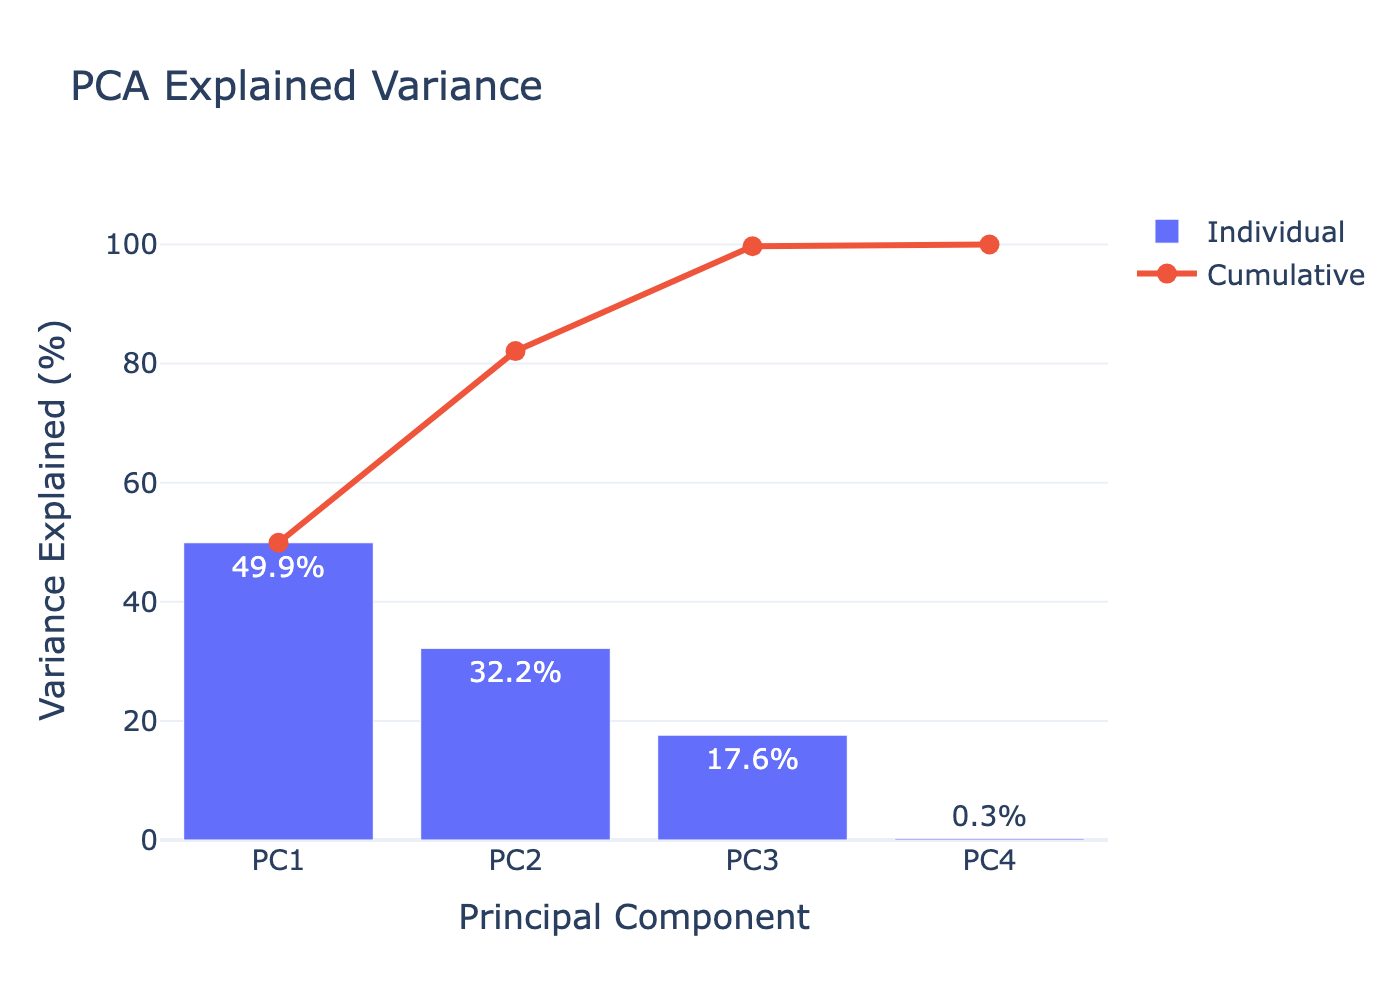
\includegraphics[width=0.85\textwidth]{figures/13_pca_scree_plot.png}
\caption{PCA Scree Plot. Three principal components explain 99.7\% of variance in weather features, with PC1 (temperature) accounting for nearly half of the total variance.}
\label{fig:pca}
\end{figure}

\subsection{Feature Importance}

Random Forest feature importance reveals the key predictors:

\begin{figure}[H]
\centering
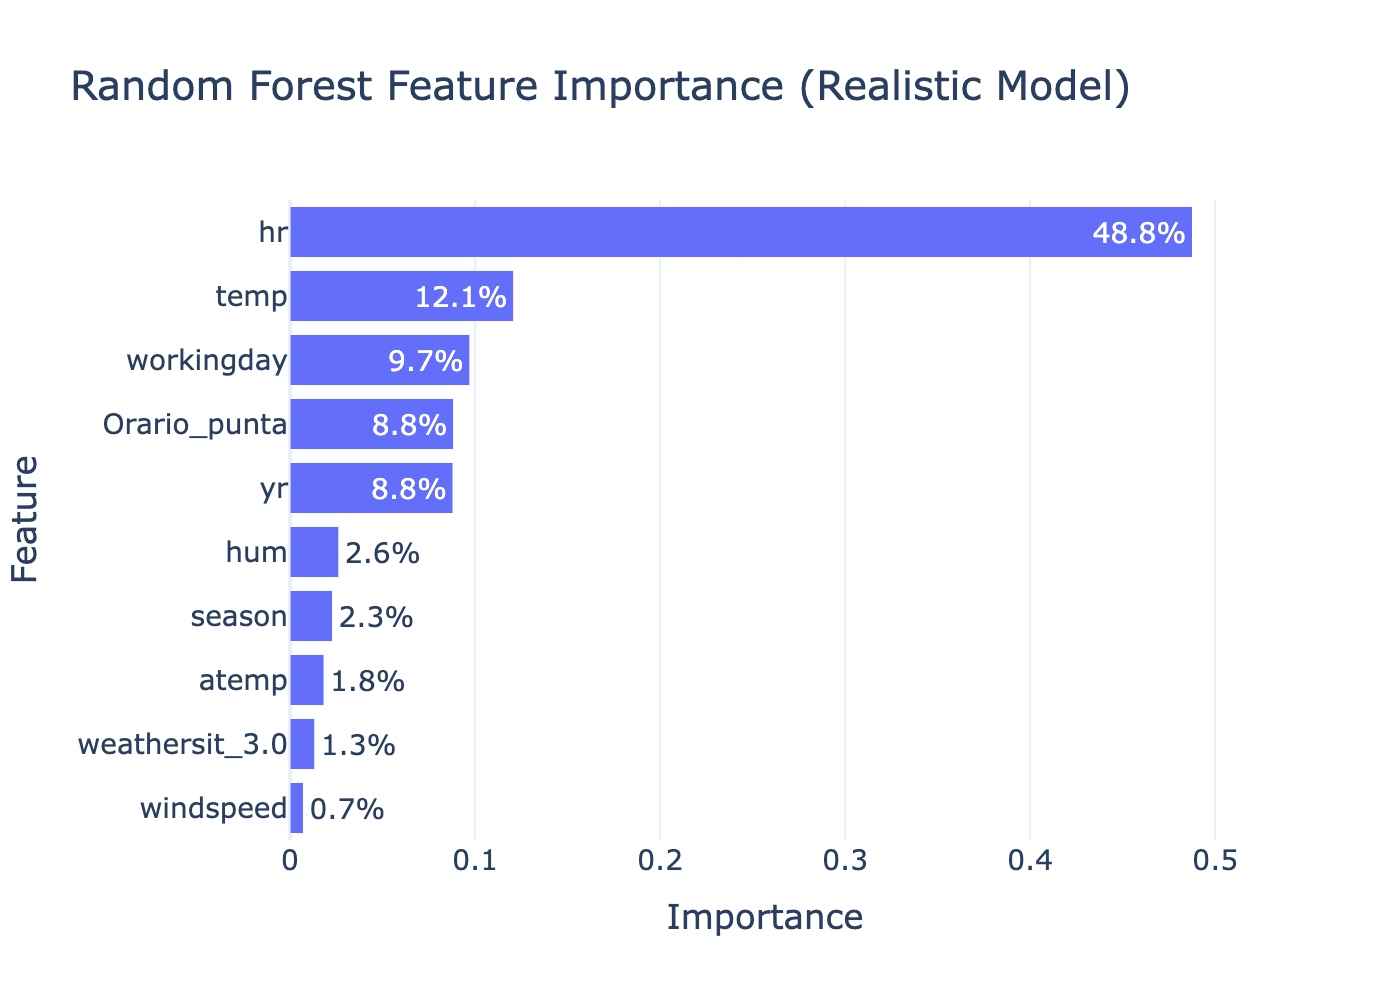
\includegraphics[width=0.85\textwidth]{figures/14_feature_importance.png}
\caption{Feature Importance Ranking. Hour of day alone accounts for approximately 48.8\% of predictive power, followed by temperature (12.1\%), working day indicator (9.7\%), and peak hour flag (8.8\%).}
\label{fig:importance}
\end{figure}

\begin{table}[H]
\centering
\caption{Top 10 Feature Importance Scores}
\begin{tabular}{clc}
\toprule
\textbf{Rank} & \textbf{Feature} & \textbf{Importance} \\
\midrule
1 & hr (hour) & 48.77\% \\
2 & temp & 12.09\% \\
3 & workingday & 9.72\% \\
4 & Orario\_punta (peak hour) & 8.84\% \\
5 & yr (year) & 8.81\% \\
6 & hum (humidity) & 2.64\% \\
7 & season & 2.30\% \\
8 & atemp & 1.84\% \\
9 & weathersit\_3.0 & 1.34\% \\
10 & windspeed & 0.73\% \\
\bottomrule
\end{tabular}
\label{tab:importance}
\end{table}

\section{Model Development}

\subsection{Data Leakage Analysis}

A critical discovery during model development was the presence of data leakage in the original feature set. The initial model achieved suspiciously perfect metrics:

\begin{table}[H]
\centering
\caption{Model Performance: Leaky vs Realistic}
\begin{tabular}{lcccc}
\toprule
\textbf{Model} & \textbf{R$^2$} & \textbf{RMSE} & \textbf{MAE} & \textbf{MAPE} \\
\midrule
Leaky Model & 0.9999 & 1.21 & 0.52 & 0.27\% \\
Realistic Model & 0.9456 & 41.01 & 25.05 & 30.65\% \\
\bottomrule
\end{tabular}
\label{tab:models}
\end{table}

\textbf{Sources of Data Leakage:}

\begin{enumerate}
    \item \textbf{Lag Features (cnt\_lag\_1 to cnt\_lag\_24)}: These features contain actual target values from previous hours, essentially giving the model direct access to the answer.

    \item \textbf{User Type Decomposition}: The features \texttt{registered} and \texttt{casual} sum exactly to \texttt{cnt} (the target variable), creating perfect multicollinearity:
    \begin{equation}
    \text{registered} + \text{casual} = \text{cnt}
    \end{equation}
\end{enumerate}

\subsection{Realistic Model Training}

The realistic model was trained excluding leaky features:

\textbf{Excluded Features:}
\begin{itemize}
    \item \texttt{cnt} (target variable)
    \item \texttt{registered}, \texttt{casual} (sum to target)
    \item \texttt{cnt\_lag\_1} through \texttt{cnt\_lag\_24} (lagged target values)
\end{itemize}

\textbf{Included Features (33 total):}
\begin{itemize}
    \item Time: hr, season, yr, workingday, holiday, Orario\_punta
    \item Weather: temp, atemp, hum, windspeed
    \item One-hot encoded: mnth\_1-12, weekday\_0-6, weathersit\_1.0-4.0
\end{itemize}

\subsection{Model Configuration}

\begin{table}[H]
\centering
\caption{Random Forest Configuration}
\begin{tabular}{ll}
\toprule
\textbf{Parameter} & \textbf{Value} \\
\midrule
Algorithm & Random Forest Regressor \\
n\_estimators & 100 \\
max\_depth & 15 \\
min\_samples\_split & 5 \\
min\_samples\_leaf & 2 \\
Train/Test Split & 80\% / 20\% \\
Test Period & December 2012 \\
\bottomrule
\end{tabular}
\label{tab:config}
\end{table}

\section{Results and Evaluation}

\subsection{Model Performance}

The realistic model achieves strong predictive performance using only weather and calendar features:

\begin{figure}[H]
\centering
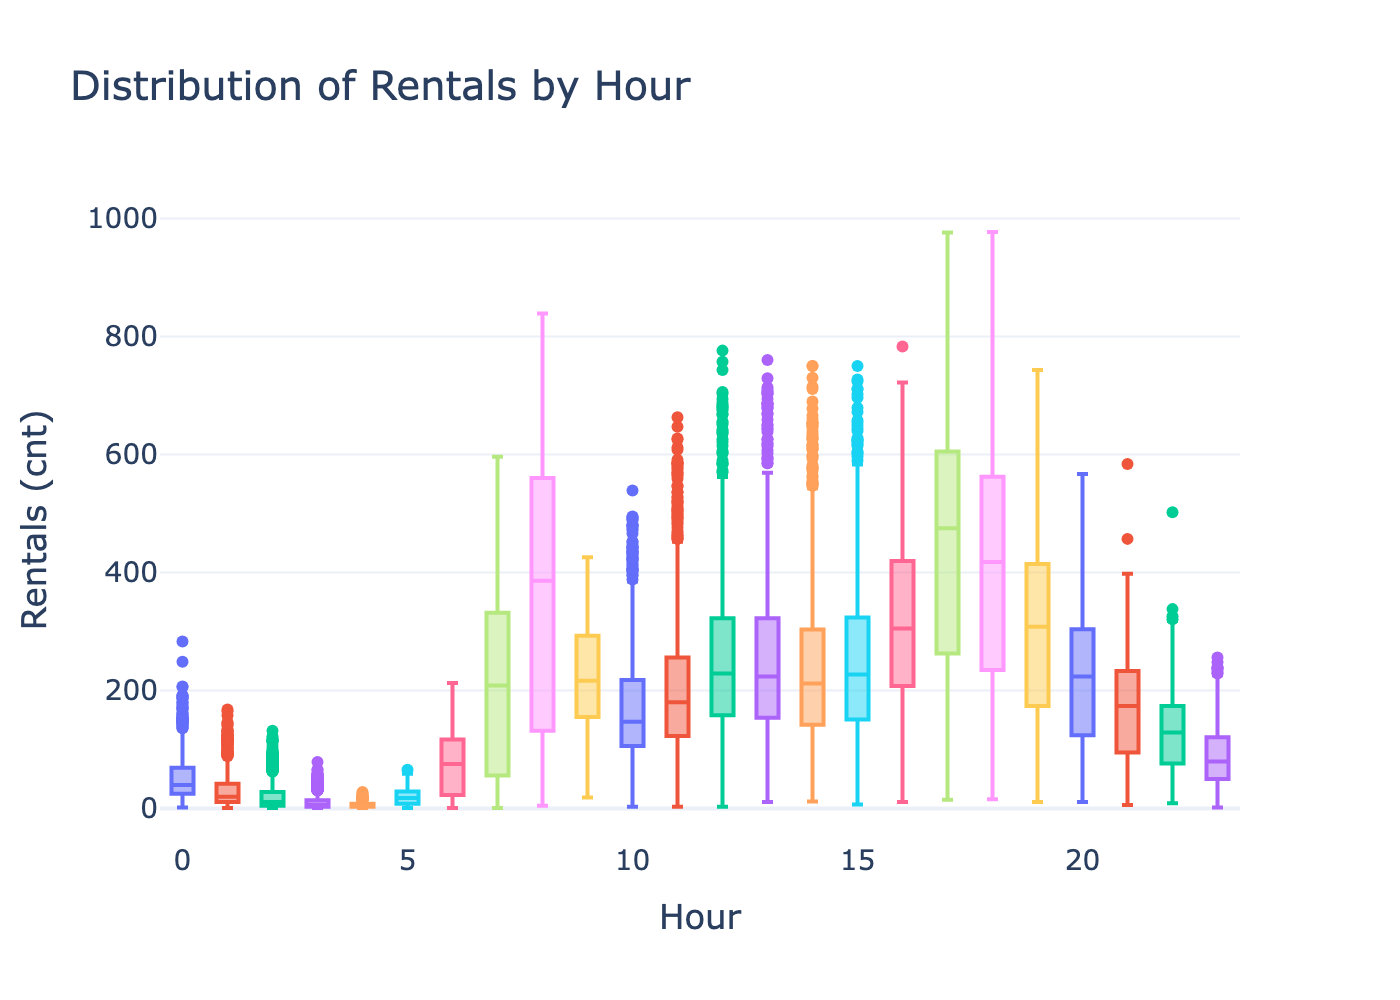
\includegraphics[width=0.85\textwidth]{figures/08_boxplot_hour.png}
\caption{Hourly Rental Distribution. Box plot showing variance in rentals across hours, with highest variability during peak commuting hours (8 AM and 5-6 PM) and minimal variance during early morning hours.}
\label{fig:boxplot}
\end{figure}

\begin{figure}[H]
\centering
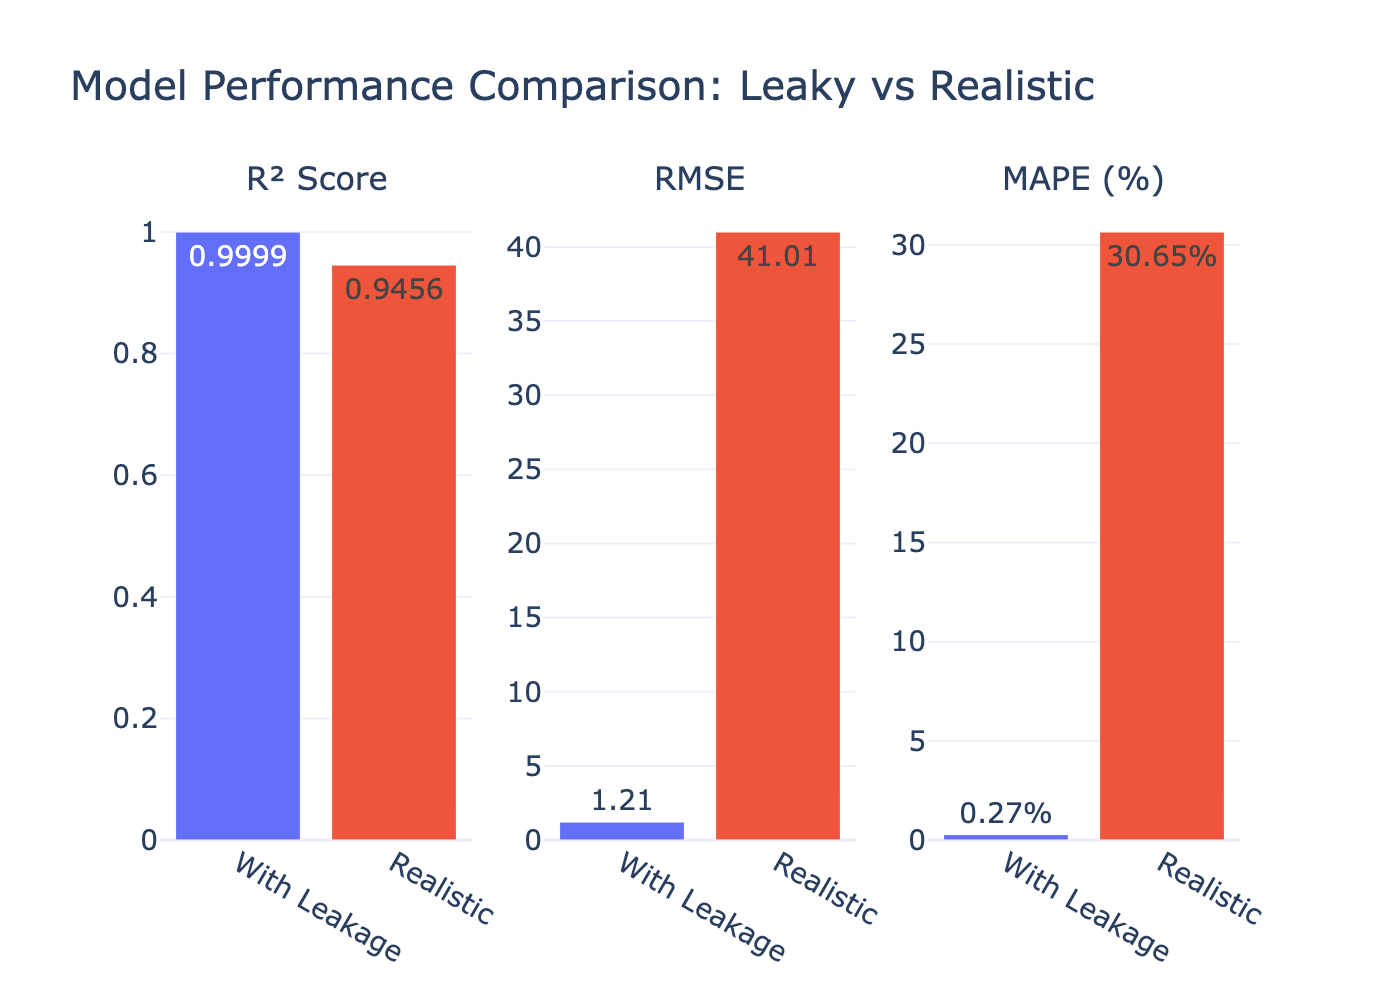
\includegraphics[width=0.85\textwidth]{figures/15_model_comparison.png}
\caption{Model Performance Comparison. Side-by-side comparison of the leaky model (R$^2$ = 0.9999) and realistic model (R$^2$ = 0.9456), demonstrating the impact of data leakage on perceived model performance.}
\label{fig:comparison}
\end{figure}

\subsection{Forecast Demonstration}

\begin{figure}[H]
\centering
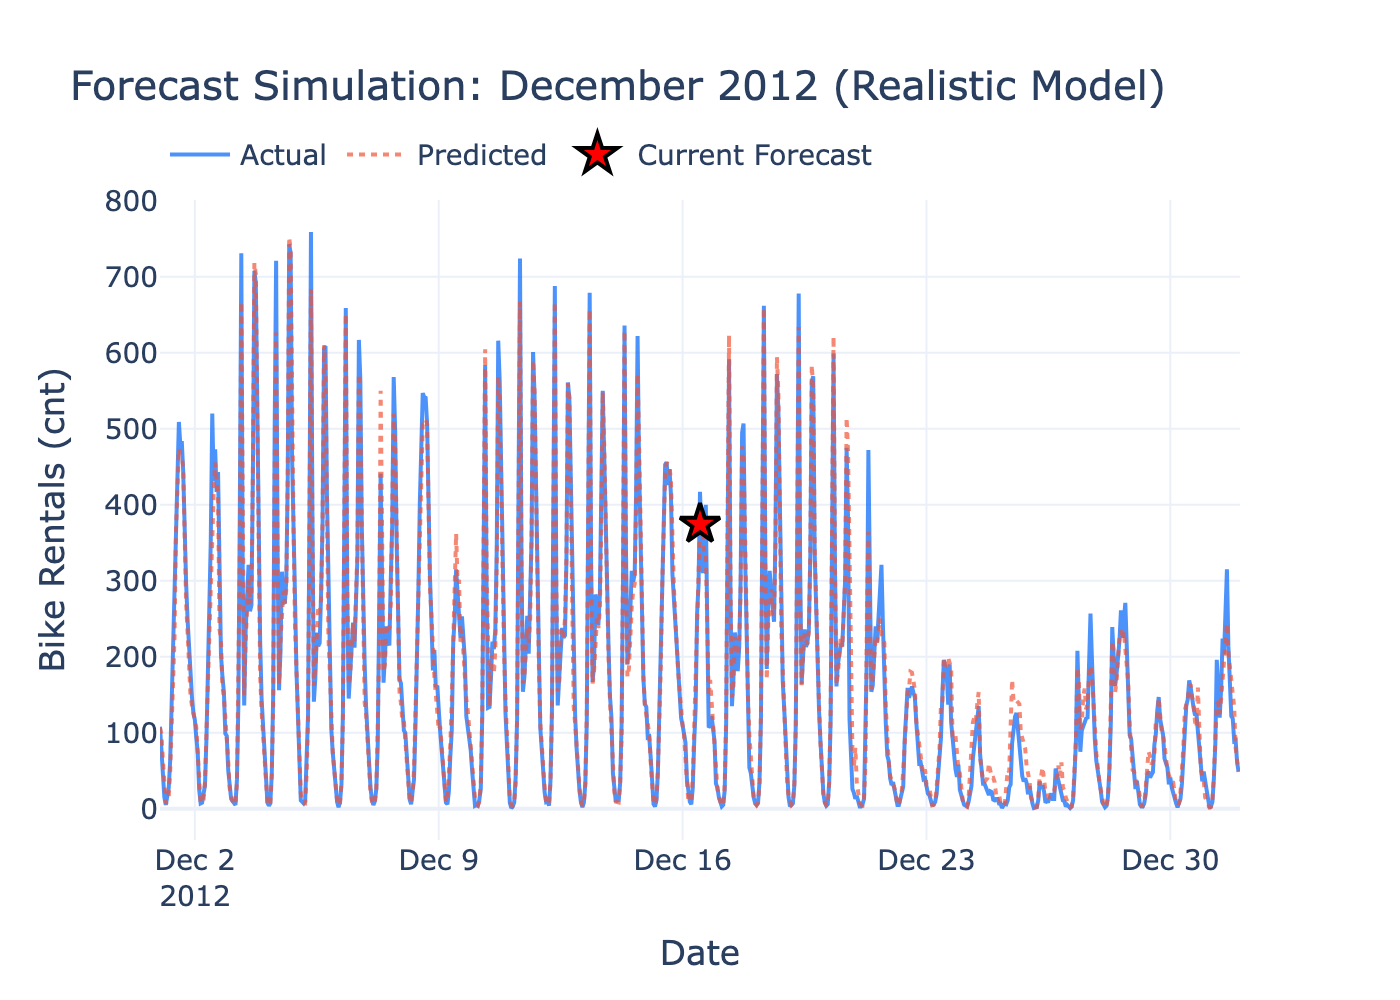
\includegraphics[width=0.85\textwidth]{figures/16_forecast_simulation.png}
\caption{Forecast Simulation (December 2012). Actual vs predicted bike rentals for the test period, showing the realistic model's ability to capture daily and weekly patterns with R$^2$ = 0.9456.}
\label{fig:forecast}
\end{figure}

\subsection{Performance Interpretation}

The realistic model's R$^2$ = 0.9456 indicates that:
\begin{itemize}
    \item The model explains \textbf{94.56\%} of variance in bike rental demand
    \item Using only weather forecasts and calendar information (available in advance)
    \item This represents achievable performance in a \textbf{real deployment scenario}
    \item An R$^2$ of $\sim$0.95 is considered \textbf{excellent} for demand forecasting
\end{itemize}

\subsection{Temperature Correlation}

\begin{figure}[H]
\centering
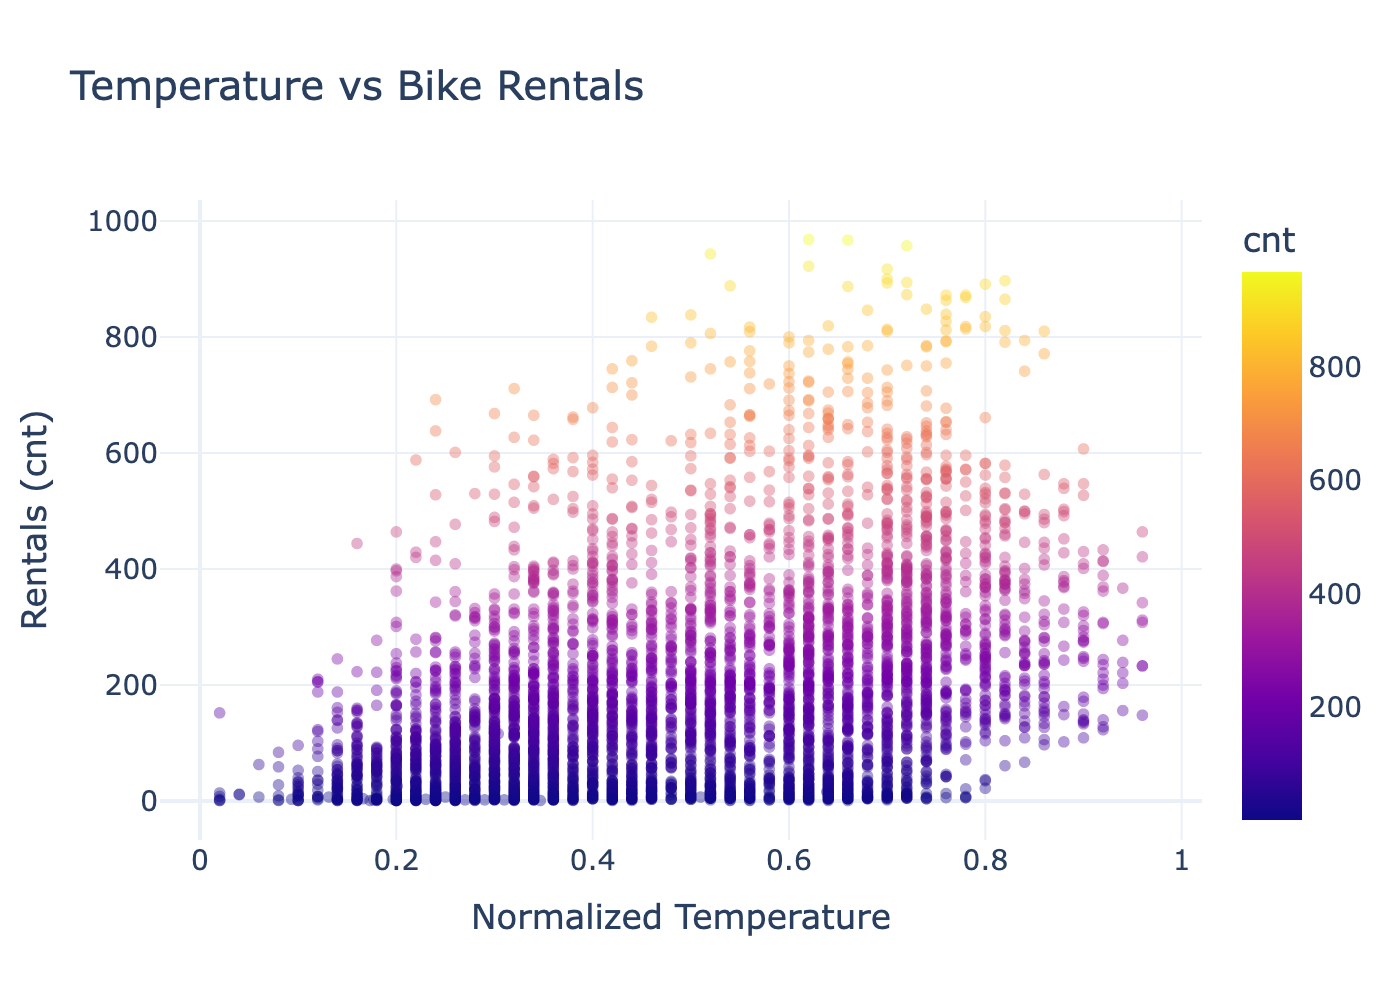
\includegraphics[width=0.85\textwidth]{figures/09_temp_vs_rentals.png}
\caption{Temperature vs Rental Correlation. Scatter plot showing positive correlation between temperature and bike rentals, with optimal rental conditions occurring between 0.5-0.8 normalized temperature range.}
\label{fig:temp}
\end{figure}

\section{Discussion}

\subsection{Key Findings}

\begin{enumerate}
    \item \textbf{Data Leakage Discovery}: The most significant finding was the identification of data leakage that inflated model performance from realistic (R$^2$ = 0.9456) to artificially perfect (R$^2$ = 0.9999). This highlights the importance of careful feature engineering in time series forecasting.

    \item \textbf{Temporal Dominance}: Hour of day alone accounts for nearly 50\% of predictive power, confirming that bike-sharing is primarily driven by commuting patterns.

    \item \textbf{User Segmentation}: The 82.5\% registered user base shows fundamentally different behavior from casual users, particularly in weather sensitivity (56.3\% vs 93.4\% storm reduction).

    \item \textbf{Strong Seasonality}: Time series decomposition and autocorrelation analysis confirm strong daily and weekly patterns suitable for forecasting.
\end{enumerate}

\subsection{Dashboard Value}

The Streamlit dashboard provides several operational benefits:
\begin{itemize}
    \item \textbf{Interactive Exploration}: Stakeholders can explore patterns without programming knowledge
    \item \textbf{Real-Time Forecasting}: Simulation interface demonstrates prediction capabilities
    \item \textbf{Model Comparison}: Multiple models can be compared side-by-side
    \item \textbf{Advanced Analytics}: Statistical methods (decomposition, ACF/PACF, PCA) accessible through intuitive interface
\end{itemize}

\subsection{Limitations}

\begin{enumerate}
    \item \textbf{Single System}: Analysis based on one bike-sharing system; generalizability to other cities uncertain
    \item \textbf{Historical Data}: Two years of data may not capture longer-term trends or rare events
    \item \textbf{Static Model}: Current implementation does not support online learning or model updating
    \item \textbf{Feature Availability}: Real-time deployment requires accurate weather forecasts
\end{enumerate}

\subsection{Lessons Learned}

\begin{enumerate}
    \item Always examine feature sets for potential data leakage before celebrating high performance
    \item User segmentation provides valuable insights beyond aggregate analysis
    \item Interactive dashboards make complex analysis accessible to non-technical stakeholders
    \item Time series decomposition helps validate forecasting model assumptions
\end{enumerate}

\section{Conclusion and Future Work}

\subsection{Summary of Contributions}

This project successfully developed a comprehensive bike rental analysis dashboard with:

\begin{enumerate}
    \item A four-page Streamlit application with interactive data exploration and forecasting
    \item Discovery and correction of data leakage that artificially inflated model performance
    \item A realistic Random Forest model achieving R$^2$ = 0.9456 for demand forecasting
    \item Comprehensive time series analysis including decomposition, ACF/PACF, and PCA
    \item Quantified insights on user segmentation and weather sensitivity
\end{enumerate}

The system demonstrates that bike rental demand can be accurately predicted (94.56\% variance explained) using only weather and calendar features available in advance.

\subsection{Future Work}

Several directions merit further investigation:

\begin{enumerate}
    \item \textbf{Deep Learning Models}: Explore LSTM and Transformer architectures for sequence modeling
    \item \textbf{Spatial Analysis}: Incorporate station-level predictions for rebalancing optimization
    \item \textbf{Real-Time Integration}: Connect dashboard to live data feeds and weather APIs
    \item \textbf{Ensemble Methods}: Combine multiple models for improved robustness
    \item \textbf{Uncertainty Quantification}: Add prediction intervals for risk-aware decision making
    \item \textbf{Anomaly Detection}: Implement alerts for unusual demand patterns
\end{enumerate}

\begin{thebibliography}{99}

\bibitem{borgnat2011shared}
Borgnat, P., Abry, P., Flandrin, P., Robardet, C., Rouquier, J. B., \& Fleury, E. (2011). Shared bicycles in a city: A signal processing and data analysis perspective. \textit{Advances in Complex Systems}, 14(03), 415-438.

\bibitem{xu2018bike}
Xu, C., Ji, J., \& Liu, P. (2018). The station-free sharing bike demand forecasting with a deep learning approach and large-scale datasets. \textit{Transportation Research Part C: Emerging Technologies}, 95, 47-60.

\bibitem{cleveland1990stl}
Cleveland, R. B., Cleveland, W. S., McRae, J. E., \& Terpenning, I. (1990). STL: A seasonal-trend decomposition. \textit{Journal of Official Statistics}, 6(1), 3-73.

\bibitem{breiman2001random}
Breiman, L. (2001). Random forests. \textit{Machine Learning}, 45(1), 5-32.

\bibitem{streamlit2024}
Streamlit Inc. (2024). Streamlit Documentation. \url{https://docs.streamlit.io/}

\bibitem{hyndman2018forecasting}
Hyndman, R. J., \& Athanasopoulos, G. (2018). \textit{Forecasting: Principles and Practice}. OTexts.

\bibitem{fanaee2014event}
Fanaee-T, H., \& Gama, J. (2014). Event labeling combining ensemble detectors and background knowledge. \textit{Progress in Artificial Intelligence}, 2(2), 113-127.

\bibitem{pedregosa2011scikit}
Pedregosa, F., et al. (2011). Scikit-learn: Machine learning in Python. \textit{Journal of Machine Learning Research}, 12, 2825-2830.

\end{thebibliography}

\end{document}
